\begin{mainquestion}{capacitorcurrent}{Capacitor Analysis}

The current $i(t)$ through a 0.5-$\mu$F capacitor is shown in the figure below. At $t = 0$, the voltage $v(t)$ is 10 V.

\begin{center}
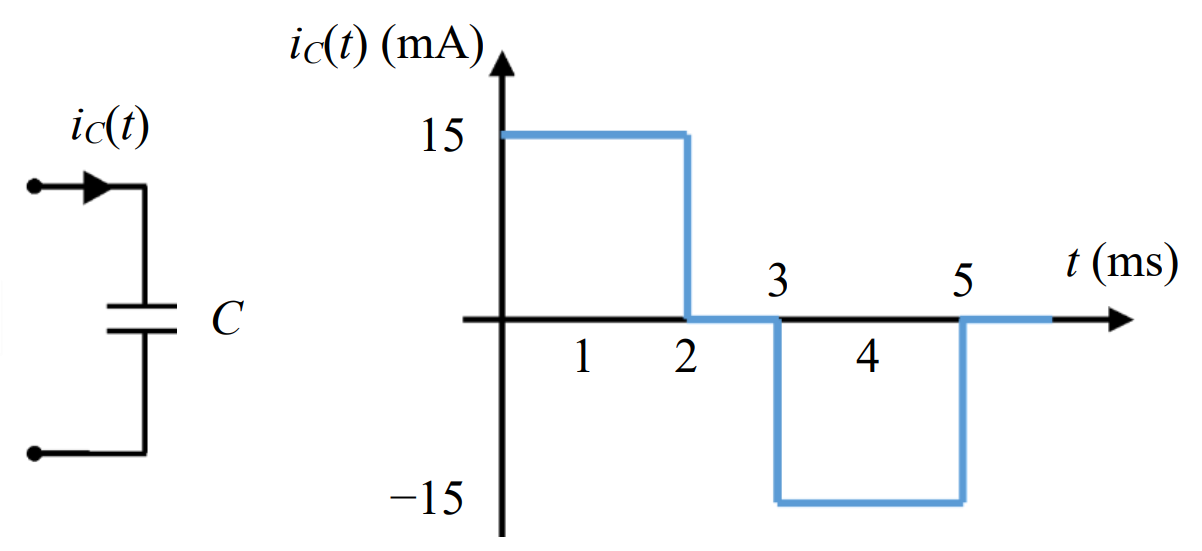
\includegraphics[width=0.8\textwidth]{questionbank/circuit_quantities/capacitor_current_energy/v0/current_circuit.png}
\end{center}

% =========================================================
\begin{partquestion}{voltagepower}
{Calculate the voltage, power, and stored energy as a function of time.}

\begin{answer}
The equation that relates the current and the voltage in a capacitor is given by:

\[
i_C(t) = C \frac{dv_C(t)}{dt} \quad \Rightarrow \quad v_C(t) = \frac{1}{C}\int i_C(t)\,dt + v_C(0)
\]

From 0 ms to 2 ms:

\[
v_C(t) = \frac{1}{0.5 \times 10^{-6}} \int_0^t 15 \times 10^{-3} \,dt' + 10 = 3 \times 10^4 t + 10 \quad (0 \leq t \leq 0.002\text{ s})
\]

At $t = 0.002$~s, $v_C(0.002) = 70$~V. Because the current becomes zero between 2 ms and 3 ms, the voltage stays constant at 70~V. From 3 ms to 5 ms the voltage in the capacitor is given by the expression below. Notice that we are using (t – 3 ms) because of the shift in time:

\[
v_C(t) = \frac{1}{0.5 \times 10^{-6}} \int_{0.003}^t -15 \times 10^{-3} \,dt' + 70 = -3 \times 10^4 (t - 0.003) + 70 \quad (0.003 \leq t \leq 0.005\text{ s})
\]

Consolidating these results gives:

\[
v_C(t) = \begin{cases}
3 \times 10^4 t + 10 & 0 \leq t \leq 0.002 \\
70 & 0.002 \leq t \leq 0.003 \\
-3 \times 10^4 (t - 0.003) + 70 & 0.003 \leq t \leq 0.005
\end{cases}
\]

The power stored is given by the product of the current and the voltage in the capacitor, that is, $p(t) = v_C(t) \cdot i_C(t)$. Therefore, (measuring power in watts):

\begin{align*}
p(t) &= \begin{cases}
(\num{3e4}t + 10)(0.015) & 0 \leq t \leq 0.002 \\
(70)(0) & 0.002 \leq t \leq 0.003 \\
(-3 \times 10^4 (t - 0.003) + 70)(-0.015) & 0.003 \leq t \leq 0.005
\end{cases} \\
&= \begin{cases}
450t + 0.15 & 0 \leq t \leq 0.002 \\
0 & 0.002 \leq t \leq 0.003 \\
450(t - 0.003) -1.05 & 0.003 \leq t \leq 0.005
\end{cases}
\end{align*}

The energy (measured in joules) stored in the capacitor is given by:

\[
E_C = \frac{1}{2} C V^2 = \frac{1}{2}(0.5 \times 10^{-6}) v_C(t)^2 = 0.25 \times 10^{-6} v_C(t)^2
\]

Using the result for the capacitor voltage from before we can determine:

\begin{align*}
E_C(t) &= \begin{cases}
\num{0.25e-6}(\num{3e4}t + 10)^2 & 0 \leq t \leq 0.002 \\
\num{0.25e-6}(70)^2 & 0.002 \leq t \leq 0.003 \\
\num{0.25e-6}(-\num{3e4}(t - 0.003) + 70))^2& 0.003 \leq t \leq 0.005
\end{cases} \\
&= \begin{cases}
225t^2 + 0.15t +\num{2.5e-5} & 0 \leq t \leq 0.002 \\
\num{1.225e-3} & 0.002 \leq t \leq 0.003 \\
225t^2 - 2.4t + \num{6.4e-3} & 0.003 \leq t \leq 0.005
\end{cases}
\end{align*}

\end{answer}
\end{partquestion}

% =========================================================
\begin{partquestion}{waveformplots}
{Plot the current, voltage, power, and stored energy to scale versus time so that the relation between each is clear.}

\begin{answer}
Plotting these graphs gives the results below:

\begin{center}
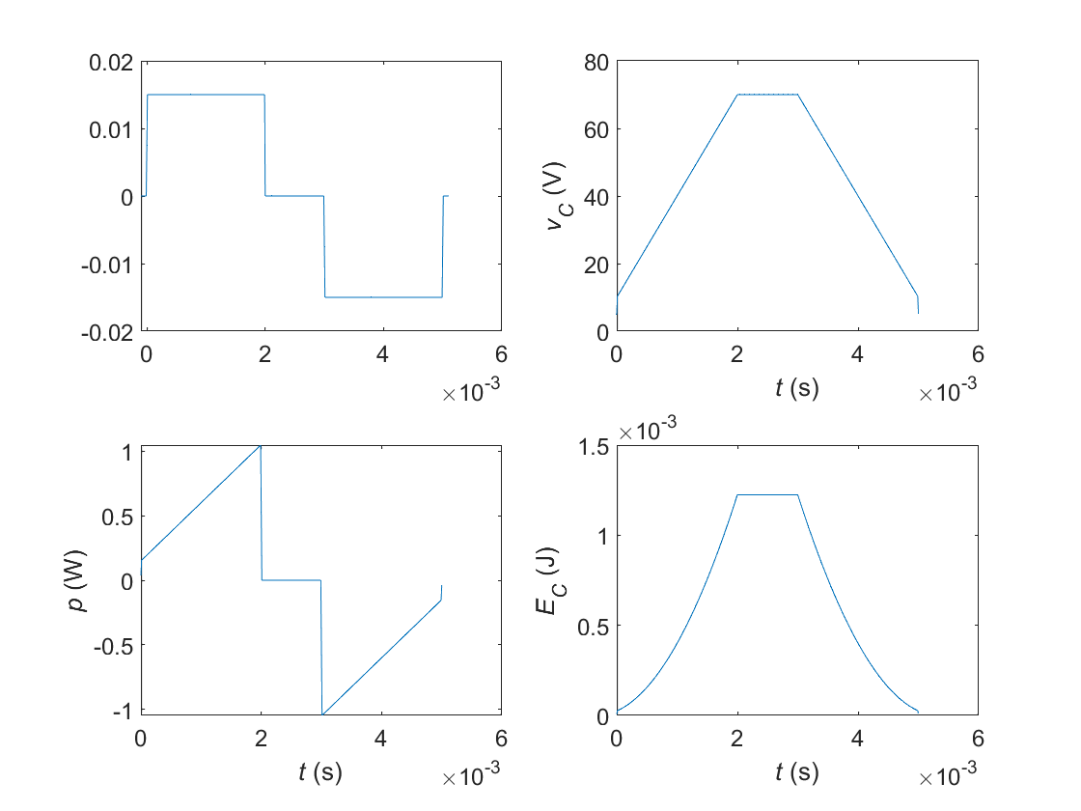
\includegraphics[width=5in]{questionbank/circuit_quantities/capacitor_current_energy/v0/waveforms.png}
\end{center}

\end{answer}
\end{partquestion}

\end{mainquestion}
